\documentclass[12pt]{article}

\usepackage[utf8]{inputenc}
\usepackage[T1]{fontenc}
\usepackage{lmodern}
\usepackage{color}
\usepackage[usenames,dvipsnames]{xcolor}
\usepackage{eurosym}
\usepackage{geometry}
\usepackage{amsmath}
\usepackage{wrapfig}
\usepackage[francais]{babel}
\usepackage[xindy,nonumberlist]{glossaries}
\usepackage{tocbibind}
\usepackage{minted}
\usepackage{url}
\usepackage{graphicx}
\usepackage{float}
\usepackage{caption}
\usepackage[table]{colortbl}
\usepackage[absolute]{textpos}
\usepackage{array}
\usepackage{appendix}

\DeclareUnicodeCharacter{00A0}{ }

\makeatletter
\def\clap#1{\hbox to 0pt{\hss #1\hss}}%
\def\ligne#1{%
\hbox to \hsize{%
\vbox{\centering #1}}}%
\def\haut#1#2#3{%
\hbox to \hsize{%
\rlap{\vtop{\raggedright #1}}%
\hss
\clap{\vtop{\centering #2}}%
\hss
\llap{\vtop{\raggedleft #3}}}}%
\def\bas#1#2#3{%
\hbox to \hsize{%
\rlap{\vbox{\raggedright #1}}%
\hss
\clap{\vbox{\centering #2}}%
\hss
\llap{\vbox{\raggedleft #3}}}}%
\def\maketitle{%
\thispagestyle{empty}\vbox to \vsize{%
\haut{}{\@blurb}{}
\vspace{1cm}

\begin{center}

\includegraphics[scale=0.2]{img/logo.jpg}
\end{center}

\vspace{1cm}
\begin{flushleft}
\usefont{OT1}{ptm}{m}{n}
\huge \@title
\end{flushleft}
\par
\hrule height 3pt
\par
\begin{flushleft}
\Large \@topic
\end{flushleft}
\par
\hrule height 3pt
\par
\begin{flushright}
\usefont{OT1}{phv}{m}{n}
\Large \@author
\par
\end{flushright}
\vspace{1cm}
\vfill
\vfill
\bas{}{\@location, le \@date}{}
}%
\cleardoublepage
}
\def\date#1{\def\@date{#1}}
\def\author#1{\def\@author{#1}}
\def\title#1{\def\@title{#1}}
\def\location#1{\def\@location{#1}}
\def\blurb#1{\def\@blurb{#1}}
\def\topic#1{\def\@topic{#1}}
\date{\today}
\author{}
\title{}
\location{Bourges}\blurb{}
\makeatother
\title{\centering\textsc{Octopus Supervisor}}
\topic{\centering\textit{Projet 4A - Supervision et audit de la sécurité système dans un réseau}}
\author{Nicolas \textsc{Cosnard} et Cyril \textsc{Segretain}}
\location{Bourges}
\blurb{%
\textbf{INSA Centre Val de Loire}\\
Département Sécurité et Technologies Informatiques\\
\textit{Année 2014-2015}\\[1em]
Responsables projet : Jérémy \textsc{Briffaut} et Martial \textsc{Szpieg}
}% 

\begin{document}
\maketitle

\renewcommand*{\glossaryname}{Lexique}
\renewcommand*{\contentsname}{Sommaire}

\section*{Remerciements}
\addcontentsline{toc}{section}{Remerciements}

\paragraph{}
Nous souhaitons remercier M. Jérémy Briffaut et M. Martial Szpieg pour leur aide lors du lancement de notre projet. Ils ont su répondre à nos questions et nous aider à nous orienter vers une solution réalisable.
\paragraph{}
Merci aussi à Charleen Plum, une artiste de talent qui a su prendre du temps pour nous proposer un superbe logo correspondant à nos attentes.
\newline https://www.behance.net/CharleenPlum
\paragraph{}
Nos remerciements vont également au Man de Linux pour son aide précieuse et sa disponibilité à toute heure. Les barbus ayant développés des plugins pour l'éditeur Vim nous ont été d'une grande aide dans ce projet qui a été quasi-intégralement développé sous Vim.

\tableofcontents{}


\section*{Introduction}
\addcontentsline{toc}{section}{Introduction}
\paragraph{}
Dans le cadre de la deuxième année d'étude du cycle ingénieur dans la formation Sécurité et Technologies Informatique de l'INSA Centre Val de Loire, nous travaillons sur un projet en binome.
Le sujet est "Supervision et audit de la sécurité système dans un réseau". Les professeurs tuteurs sur ce projet sont M. Briffaut et M. Szpieg.
\paragraph{}
L'objectif est donc de réaliser un logiciel maitre/esclave avec des fonctionnalités de supervision des esclaves et de gestion à distance de ceux-ci. 
La supervision et la gestion attendue concernent la sécurité des systèmes esclaves afin de pouvoir certifier la fiabilité des clients, la confidentialité des données, la tracabilité des communications et un système informatique sain pour l'entreprise.
\paragraph{}
Le cahier des charges demande donc un outil d'administration qui sera utilisé par des administrateurs réseaux ou des responsables sécurité d'entreprise. 
C'est un outil qui sera facilement déployable sur un parc informatique important et diversifié. Les fonctionnalités d'administration et de supervision des machines clientes seront avancées et pourront se faire de manière pratique via une interface Web.
\paragraph{}
Ce rapport vous présente de manière vulgarisée le fonctionnement de notre logiciel. Nous avons choisi de présenter le fonctionnement général du programme dans un premier temps. 
Ensuite, nous expliciterons les algorithmes de fonctionnement du serveur puis du client. Et enfin, nous présentons un peu plus en détail les points de sécurité de notre logiciel qui sont importants.
\paragraph{}
Nous proposons donc une solution légère mais offrant de nombreuses fonctionnalités permettant la supervision et l'audit de la sécurité des systèmes dans un réseau. 
Nous vous proposons une solution fiable, sécurisée et facile d'accès. Vous pourrez la découvrir dans ce rapport.

\section{Fonctionnement}
\paragraph{}
Ce projet est issu d'un besoin de supervision et d'audit sécurité système dans le réseau d'une entreprise d'aujourd'hui.
\subsection{Objectif}
\paragraph{}
Octopus a pour objectif d'être un outil d'administration réseau répondant à un besoin de gestion d'un parc informatique par un administrateur réseau. 
\paragraph{}
Le nom du projet vient de la pieuvre qui a une tête qui contient le cerveau et qui dirige le reste de son corps, et les nombreuses tentacules de celle-ci qui ne sont que l'éxécution des commandes du cerveau (« brain ») et fait remonter des informations à ce « brain ». 
L'idée est donc d'avoir un point de contrôle central pour l'administrateur qui est le « brain » et ensuite chaque poste du parc informatique correspond à une tentacule (« tentacle »). 
\paragraph{}
L'outil d'administration que nous proposons permet de connaître en temps réel le statut de connexion au réseau des postes distants et de pouvoir lancer des scripts sur ces machines distantes. Les résultats des scripts sont disponibles sur le poste d'administration. Nous pouvons alors connaître à un moment donné l'état d'utilisation du disque dur d'un poste, l'état des processus lancé sur un autre poste, … La gestion du serveur est faite à travers une interface Web accessible avec des identifiants pour l'administrateur. Depuis cette interface, nous pouvons gérer le parc, ajouter de nouvelles machines, voir l'état du parc, commander l'éxécution de scripts sur les hôtes distants.
\paragraph{}
Le serveur est multi-client et permet donc la gestion d'un parc informatique important. L'administrateur peut créer des scripts afin de ne gérer que les informations dont il juge importante pour son parc. Un échantillon de script de base est installé par défaut dans le package client.


\subsection{Algorithme}

\paragraph{}
Dans un premier temps, nous avons travaillé sur un algorithme de notre solution afin de montrer le fonctionnement et les points-clés de celle-ci.
\paragraph{}
Les fonctionnalités maitre/esclave que présente Octopus Supervisor sont :
\begin{itemize}
 \item Ajout de nouveaux esclaves
 \item Gestion des esclaves
 \item Envoi de scripts aux esclaves
 \item Réception et stockage de résultats de scripts sur le serveur
\end{itemize}

\begin{figure}[!h]
    \centering
    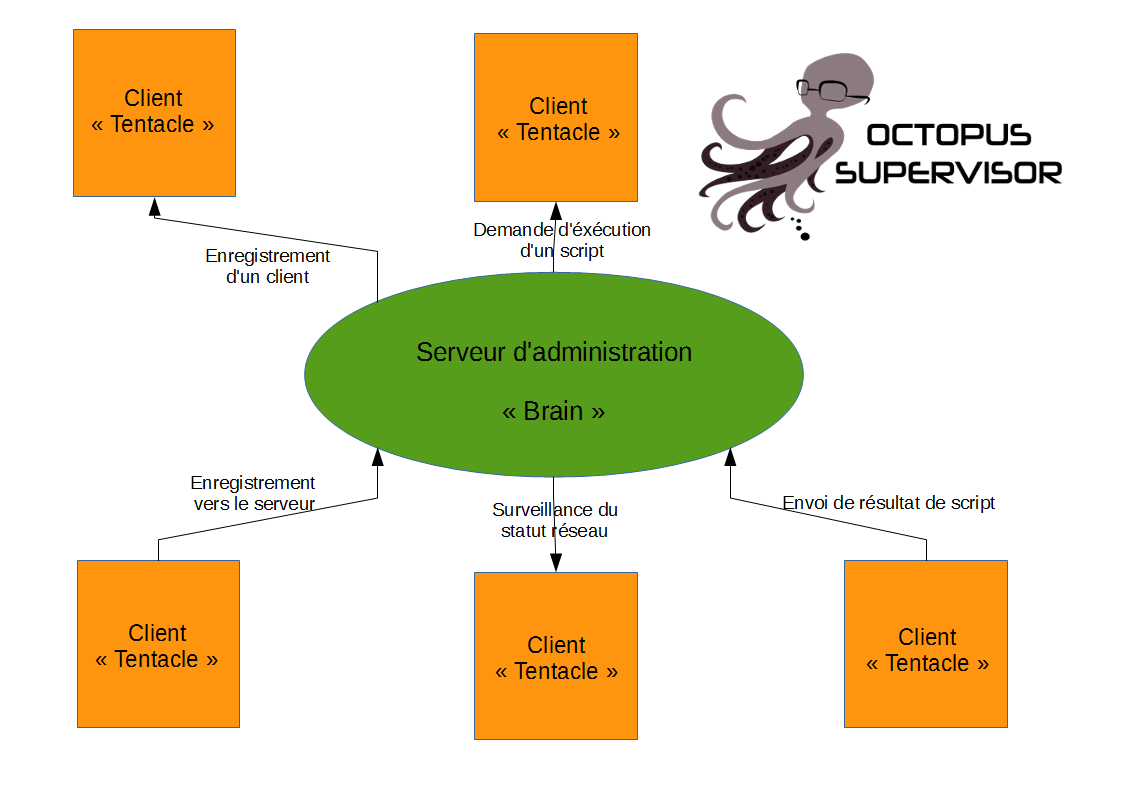
\includegraphics[width=\textwidth]{img/algo_general.png}
    \caption{Algorithme général de fonctionnement de Octopus Supervisor}
\end{figure}

\paragraph{}
Ci-dessous, un algorithme explicite techniquement le fonctionnement général de Octopus Supervisor.
\paragraph{}
Les deux entités maitre et esclave communiquent sur le réseau grâce à leur adresse IP et un port défini suivant le type de communication. Lors de l'enregistrement d'un client, le serveur est réceptif sur le port 6000. Si le client n'a pas de serveur spécifié lors de son lancement, il va attendre une communication sur le port 7000 de la part d'un serveur.
\begin{figure}[!h]
    \centering
    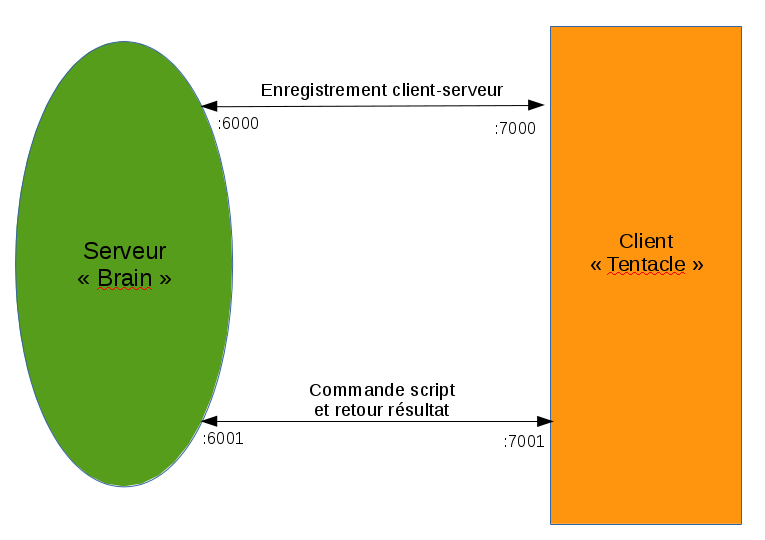
\includegraphics[width=\textwidth,height=9cm,keepaspectratio=true]{img/fct.png}
    \caption{Fonctionnement}
\end{figure}

\section{OctoBrain}

\paragraph{}
La partie de notre projet appelé OctoBrain est en fait la partie serveur d'administration. C'est le cerveau du logiciel qui contrôle les hôtes et permet la supervision et l'audit du parc.

\subsection{Algorithme}
\paragraph{}
Le maestro est le chef d'orcheste de notre logiciel, il coordonne le serveur et ses différents threads.
Nous avons choisi de diviser les actions du serveurs en plusieurs threads :
\begin{itemize}
    \item le serveur Web qui interagit avec l'administrateur via une interface Web. Le serveur est entièrement codé en C, il permet d'afficher des pages HTML et du Javascript.
    \item un registerer, qui signifie « enregistreur ». Celui-ci permet d'écouter sur le port 6000 si un client souhaite s'enregistrer sur le serveur, et il permet aussi d'ajouter manuellement des clients grâce à leur adresse IP.
    \item un commander qui permet la gestion des commandes sur le serveur. Il peut envoyer des commandes aux clients et recevoir les résultats.
\end{itemize}

\begin{figure}[h]
    \begin{center}
        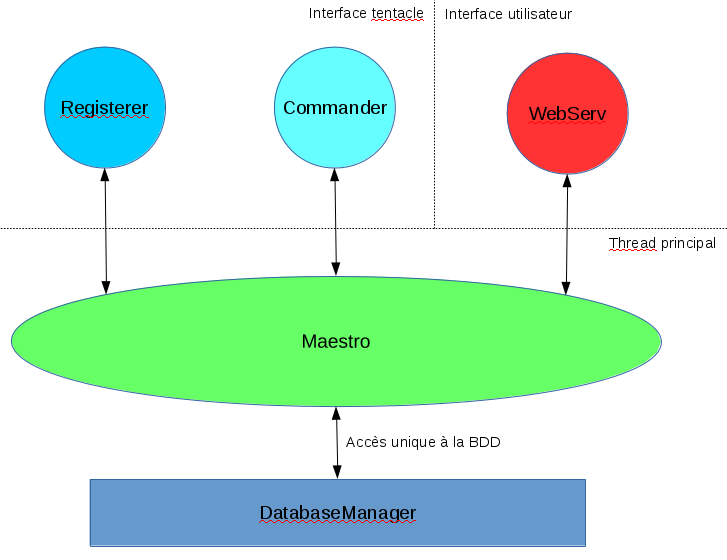
\includegraphics[height=8cm, keepaspectratio=true]{img/algo_brain_full.png}
        \caption{Fonctionnement technique du Brain}
    \end{center} 
\end{figure}

\paragraph{}
L'architecture que nous avons développé pour le Brain reprend une architecture MVC (Modèle-Vue-Contrôleur). Ce type de fonctionnement permet de bien organiser son code source et de séparer facilement les rôles entre les processus du serveur.
Le côté Modèle se retrouve dans le dbManager, la partie Vue est représenté par les différentes interfaces et le Contrôleur correspond au Maestro.

\subsection{Maestro}
\paragraph{}
Le logiciel coté serveur est orchestré autour d'un processus appelé « Maestro ». Son rôle est de coordonner les différents processus que peut lancer le serveur. Ces processus sont des forks permettant de communiquer de manière indépendante avec les clients. 
Le maestro joue un rôle indispensable dans notre logiciel car il est l'interface de communication avec la base de données du serveur. C'est le seul accès permettant de lire et écrire en base de données. En effet, généralement, les bases de données peuvent accepter les accès multiples en lecture mais un accès unique en écriture. Nous avons donc créé ce maestro afin de coordonner tous les liens avec la base de données.
Le maestro est en écoute constante sur des pipes reliés aux différentes parties du serveur. Le contrôle d'accès peut se faire en un point unique grâce à ce Maestro.

\subsection{WebServ}
\paragraph{}
Le WebServ de Octopus permet l’administration du serveur à distance par l’administrateur. 
Ce serveur web permet de voir et d’ajouter les clients, d’envoyer des instructions de scripts aux clients et aussi d’afficher les résultats des scripts éxécutés. 
Le WebServ est l'interface de manipulation des données contenues en base de données. 
\paragraph{}
Le serveur Web est un daemon écrit en C qui permet de lire et d’envoyer des fichiers (HTML, CSS, JavaScript, images) et du texte JSON. 
Le site est formé d'une unique page HTML, dont le contenu est modifié dynamiquement grâce à du javascript et des appels AJAX. 
Les interactions avec des boutons et liens déclenchent des requêtes GET avec différents arguments, et le serveur Web retourne du JSON avec les données demandées. 
Cela permet un contenu dynamique, tout en minimisant les échanges réseau.


\subsection{DbManager, Registerer et Commander}
\paragraph{}
Le DatabaseManager est le gestionnaire de fonctions de lecture et d'écriture dans la base de données. Le logiciel utilise Sqlite3 comme base de données. L'avantage est la facilité d'utilisation de Sqlite3 et il ne demande que peu de ressources matérielles. 
Afin d'accéder en lecture et écriture sur les différentes tables de la base de données, nous avons recréé des fonctions spécifiques.
\paragraph{}
Le Registerer est le daemon d'enregistrement des clients. Il est composé de deux fonctions principales. 
Une première qui est un socket en écoute permanente sur le port 6000 dans le cas ou un Tentacle rejoindrait le réseau et aurait l'adresse IP du Brain. Lorsqu'un nouveau Tentacle tente de contacter le Brain sur le port 6000, celui-ci lance l'enregistrement du Tentacle.
La seconde fonction est appelé lorsque l'administrateur du réseau ajoute manuellement une nouvelle machine sur le réseau. 
L'ajout de la nouvelle machine se fait en fournissant l'adresse IP, ensuite le Brain prend en charge de contacter le client sur le port 7000 pour avoir les informations complémentaires permettant l'enregistrement.
\paragraph{}
Le Commander est le troisième fork qui est en fonctionnement sur le serveur. Celui-ci permet d'envoyer des commandes aux clients et de recevoir les résultats des scripts. 
Ce service se lance lorsque l'administrateur demande à lancer un script sur un Tentacle à travers le WebServ ou quand un Tentacle a terminé l'éxécution d'un script et veut envoyer le résultat de celui-ci au serveur. 
Le Commander peut donc ouvrir une socket vers le client sur le port 7001 pour l'envoi d'une commande, il se déconnecte ensuite. Le Commander est également en écoute sur le port 6001 du Brain et quand un Tentacle se connecte pour envoyer des données, il sauvegarde le rapport en base de données.
\section{OctoTentacle}
\paragraph{}
La partie OctoTentacle de notre logiciel est le côté client. C'est un module qui est installé sur un hôte afin de pouvoir être superviser et auditer par le serveur.

\subsection{Algorithme}
\paragraph{}
Le client est divisé en deux parties principales : une partie pour l'enregistrement du client auprès du serveur et une partie qui permet d'interagir avec le serveur pour l'éxécution des scripts et l'envoi des rapports.

\begin{figure}[!h]
    \begin{center}
        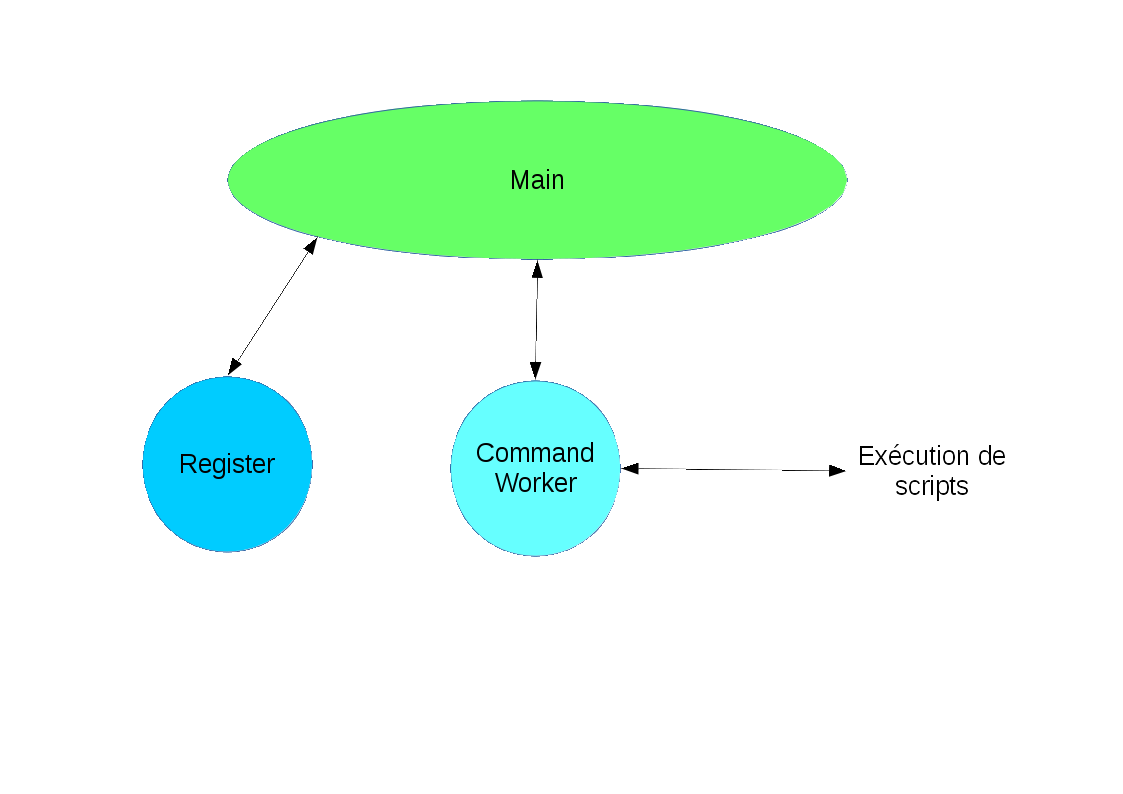
\includegraphics[width=1\textwidth]{img/algo_tentacle.png}
        \caption{Fonctionnement technique du Tentacle}
    \end{center} 
\end{figure}

\subsection{Register}
\paragraph{}
La partie enregistrement du client possède deux fonctions : une première fonction qui est un daemon et attend qu'un serveur d'administration le contacte pour proposer un enregistrement sur le réseau, une seconde fonction qui est à l'initiative de l'enregistrement auprès du brain en connaissant son adresse IP. 
Le daemon d'enregistrement écoute sur le port 7000. Lorsqu'un serveur souhaite enregistrer le client sur son réseau, il y a un échange d'informations. Le client donne son hostname, le serveur lui fournit  un ID et une clé générée par le brain et qui permettra de sécuriser l'authentification entre le client et le serveur. Une fois l'enregistrement terminé, le thread se termine et un nouveau thread se lance, le daemon de scripts.
Si lors de son lancement le client a en paramètre l'adresse IP d'un serveur avec l'option -b, le client va alors contacter directement le serveur pour demander à être enregistrer. L'enregistrement se fait ensuite de la même manière.

\subsection{CommandWorker}
\paragraph{}
Le CommandWorker est un processus du Tentacle qui permet la réception des demandes d'éxécution de script de la part du Brain, l'éxécution de ces commandes et l'envoi des résultats vers le Brain.
\paragraph{}
Dans un premier temps, le Tentacle se place en écoute sur le port 7001. Quand le Brain auquel il est affilié se connecte sur ce socket, il y a authentification des parties et le Brain demande au Tentacle d'éxécuter un script qu'il possède. 
La connexion se ferme ensuite. Le Tentacle éxécute alors le script demandé en local et sauvegarde le retour du script dans un fichier en local. 
Une fois le fichier sauvegardé en local, le Tentacle va initier une connexion avec le Brain sur le port 6001 en demandant la sauvegarde du résultat du script en base de données.
Le contenu du fichier est donc envoyé au Brain et le résultat sera ensuite accessible pour l'administrateur via l'interface Web.
\section{Approfondissement technique sur la sécurité}
\paragraph{}
Cette section du rapport rassemble des points plus technique concernant Octopus Supervisor. Elle met en avant les points d'honneur fait sur la sécurité du logiciel.

\subsection{SSL}
\paragraph{}
Dès le lancement du projet, nous avions décidé que le client et le serveur échangerait des données chiffrées par SSL. 
Toutes les communications à travers des sockets utilisent le protocole SSL (Secure Socket Layer). Nous avons donc auto-signé un certificat pour le serveur.
Une authentification SSL est effectuée à chaque ouverture de socket entre les extrémités serveur et client.
\paragraph{}
Les échanges du serveur Web se font aussi avec le protocole SSL, nous avons donc une sécurisation des commandes de l'administrateur depuis l'interface Web.
Ceci nous permet d'assurer la confidentialité des données de bout en bout lors des communication entre des entités.

\subsection{Handshake}
\paragraph{}
Octopus Supervisor travaille avec un serveur et plusieurs clients. Afin de savoir avec qui l'on communique, il y a une phase d'authentification au début d'un échange entre deux entités.
Cette authentification est appelée "handshake", signifiant poignée de main. Elle commence par un message initiant la communication puis un acquittement. Ensuite il y a un échange d'ID pour identifier le Tentacle.
La dernière étape du Handshake est de vérifier la clé correspondant à l'ID qui a été générée lors de l'enregistrement du Tentacle sur le Brain.

\begin{figure}[!h]
	\centering
	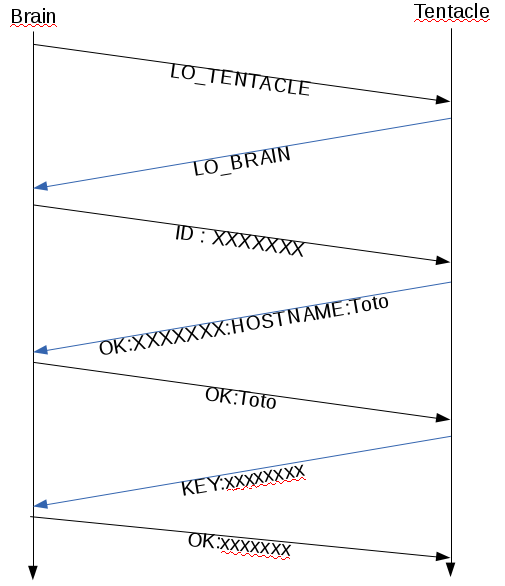
\includegraphics[scale=0.55]{img/handshake_register_btot.png}
        \caption{Handshake enregistrement}
\end{figure}

\paragraph{}
La Figure 5 représente l'initialisation de la communication entre le Brain et un Tentacle lors de l'enregistrement du dernier sur le Brain. Quand le Brain reçoit une adresse IP à ajouter à sa base de données, la communication suivante est effectuée.

\begin{figure}[!h]
	\centering
	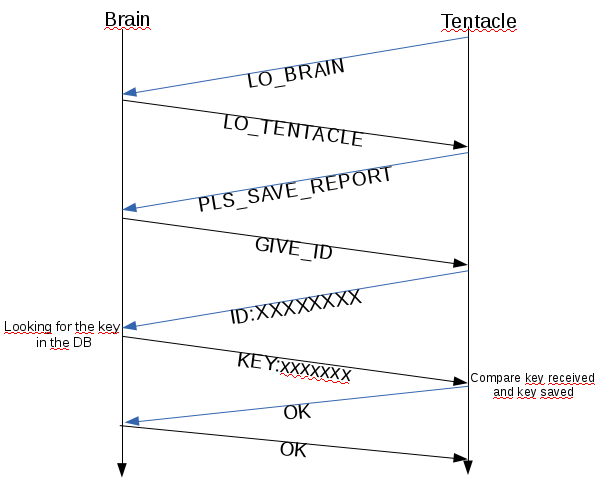
\includegraphics[scale=0.6]{img/handshake_commander_ttob.png}
	\caption{Handshake envoi résultat}
\end{figure}

\paragraph{}
La Figure 6 présente le handshake qui est fait lorsqu'un Tentacle contacte le Brain pour envoyer un résultat de script.
\paragraph{}

\subsection{Timeout web}
\paragraph{}
L'utilisation de Octopus Supervisor se fait grâce à une interface Web. Celle-ci nécessite une connexion avec un login et un mot de passe pour pouvoir identifier les administrateurs du logiciel.
Lorsqu'un utilisateur du logiciel se connecte à l'interface Web, une clé de session est créée et un timer est lancé. Si au bout de 300 secondes, l'utilisateur n'a pas interagi avec le WebServ, la clé de session ne sera plus valide et l'utilisateur sera automatiquement déconnecté.
Cela permet d'éviter une connexion permanente qui expose aux risques d'usurpation d'identité par session d'utilisateur.

\section{Bilan}

\subsection{Difficultés rencontrées}
\paragraph{}
Au cours de ce projet, nous avons rencontrées plusieurs difficultés, certaines humaines et d'autres techniques.
\paragraph{}
D'une part, la gestion de projet a été faite de manière approximative car nous n'étions que deux sur le projet. Cela a été un avantage mais aussi un inconvénient qui était de ne pas avoir de suivi régulier sur les tâches à effectuer.
\paragraph{}
D'autre part, sur le point de vue technique, nous nous sommes heurtés à des problèmes d'interprétation de commande SSL. Lorsqu'un message commençait par "R", OpenSSL considérait que c'était une commande qui lui est propre. Nous avons donc modifié nos messages.
\paragraph{}
L'envoi des résultats de scripts a été compliqué à mettre en place puisque nous avons souhaité mettre le contenu du fichier dans un buffer de taille dynamique pour l'envoi, la réception et la sauvegarde en BDD.
La gestion des buffers a été complexe mais fonctionne correctement aujourd'hui.

\subsection{Axes d'améliorations}
\paragraph{}
Octopus Supervisor est un logiciel fonctionnel mais auquel nous pourrions rajouter beaucoup de fonctionnalités. Parmi celles qui seraient intéressantes, nous avons retenus :
\begin{itemize}
 \item Gestion des utilisateurs depuis l'interface Web
 \item Utilisation de fichier de configuration pour le serveur et les clients
 \item Gestion d'un "KeepAlive" sur les Tentacles grâce à un ping Brain vers Tentacle
 \item Modification et suppression des scripts via l'interface Web
 \item Optimisation du WebServ et sécurisation avancée de celui-ci
\end{itemize}
Toutes ces fonctionnalités seraient une vraie valeur ajoutée pour notre logiciel. Elles sont dans l'idées d'approfondir la supervision des clients et de faciliter la gestion pour l'administrateur.

\subsection{Bilan technique}
\paragraph{}
Sur le plan des compétences technique, nous avons beaucoup appris durant ce projet. Nous avons approfondi nos connaissances dans les langages C, Javascript et JSON surtout. Git a été un outil très important dans la réalisation de notre projet.
Nous avons également pu faire une utilisation poussée de l'éditeur Vim et de ses capacités de développement.

\subsection{Bilan humain}
\paragraph{}
Sur le plan humain, ce projet nous a permis d'améliorer nos compétences de travail en groupe. Nous avons également pu mettre en pratique des connaissances de gestion de projet acquises au cours de notre formation.


\section*{Conclusion}
\addcontentsline{toc}{section}{Conclusion}
\paragraph{}
Octopus Supervisor est donc un outil de supervision et d'audit de la sécurité système dans un réseau qui est fonctionnel et prêt au déploiement. 
L'outil a les fonctionnalités correspondant au cahier des charges établi au départ avec des aspects en plus tel que la portabilité du logiciel.
\paragraph{}
C'est un outil permettant à des utilisateurs (administrateurs réseaux le plus souvent ou responsable sécurité des SI) de superviser en temps réel un parc de machines clientes. 
Cette supervision passe par l'éxécution à distance de script sur les clients afin de déceler des failles systèmes dans le parc.
\paragraph{}
Notre solution rassemble la fiabilité du logiciel qui possède un code robuste, la confidentialité car le logiciel est sécurisé sur de multiples points, la tracabilité puisque la base de données sauvegarde tous les résultats de script et des logs sont sauvegardés et l'intégrité des données car celles-ci sont chiffrées de bout en bout lors des communications.
Octopus Supervisor est une solution légère et facilement implémentable sur des systèmes à faibles performances. Ainsi, les administrateurs pourront superviser une grande diversité d'hôtes à travers leur parc informatique.
\paragraph{}
Le logiciel que nous présentons est complètement fonctionnel mais peut être améliorer afin de correspondre à des besoins plus précis suivant les entreprises. 
Un administrateur pourrait souhaiter une interface différente d'une interface Web et notre code est prêt à recevoir une nouvelle interface avec peu de modifications.
\appendix
\chapter{\textbf{\Large ANNEXES}}

\newpage

\section{Installation des Machines Virtuelles}

\subsection{Installation d'une Debian Minimale}
\paragraph{}
Ce chapitre va présenter l'installation d'une machine virtuelle sous le système d'exploitation Debian. Nous vous proposons de suivre une installation minimale, sans connexion réseau.

\begin{figure}[h]
\centering
 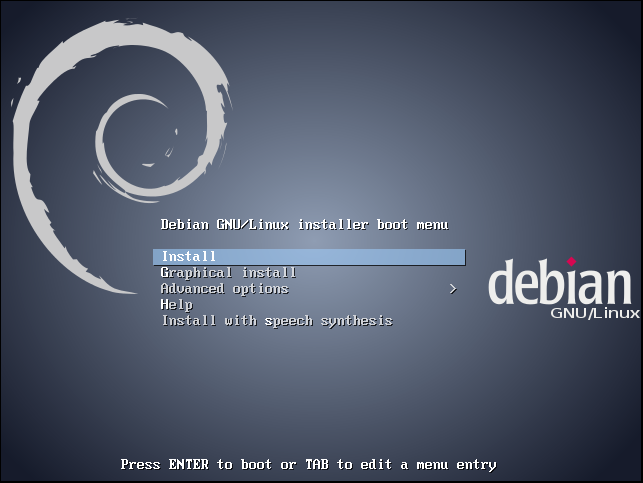
\includegraphics[scale=0.5]{img/install/Deb_inst_1.png}
 \caption{Ecran d'accueil pour l'installation de Debian}
\end{figure}
\begin{figure}[h]
 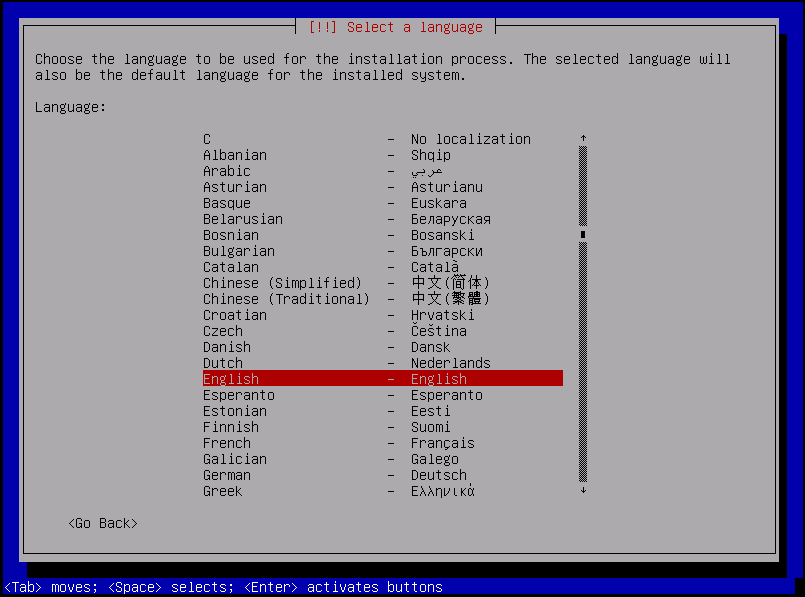
\includegraphics[scale=0.35]{img/install/Deb_inst_2.png}
 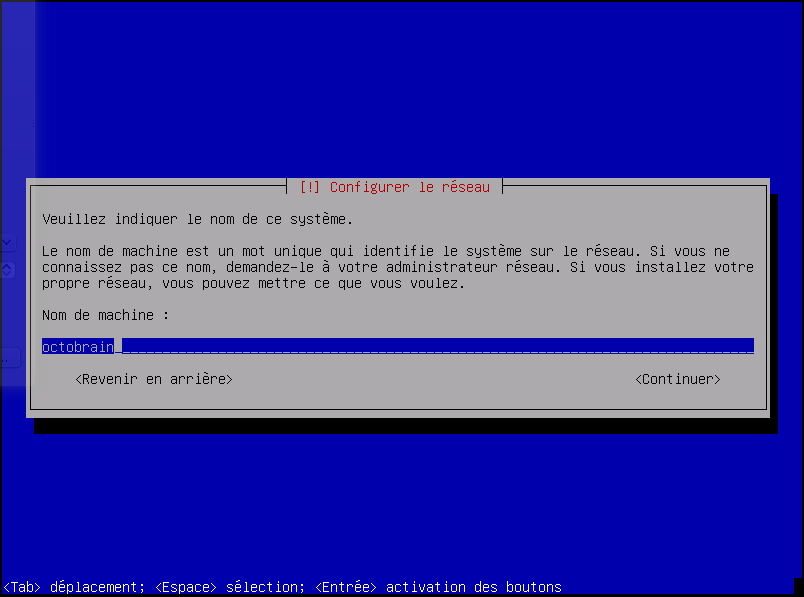
\includegraphics[scale=0.35]{img/install/Deb_inst_5.png}
 \caption{Choix de la langue et configuration réseau}
 \end{figure}
\begin{figure}
 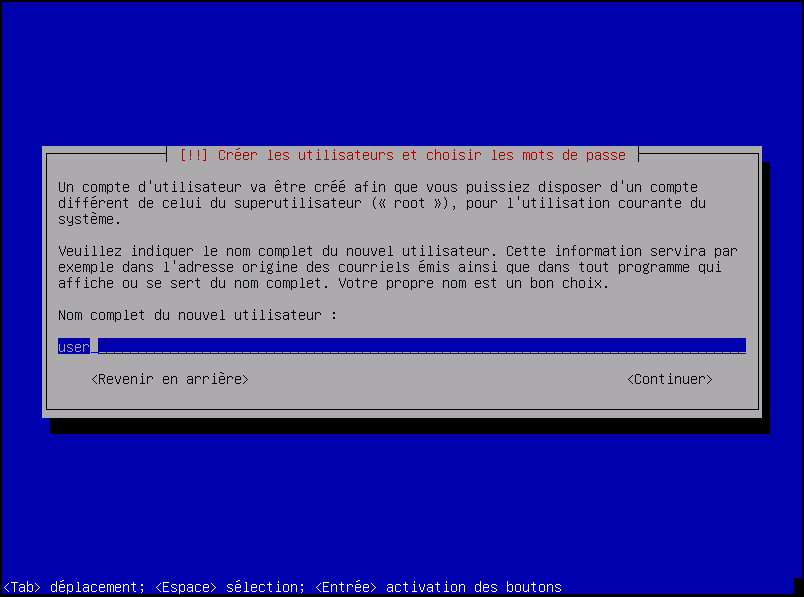
\includegraphics[scale=0.35]{img/install/Deb_inst_7.png}
 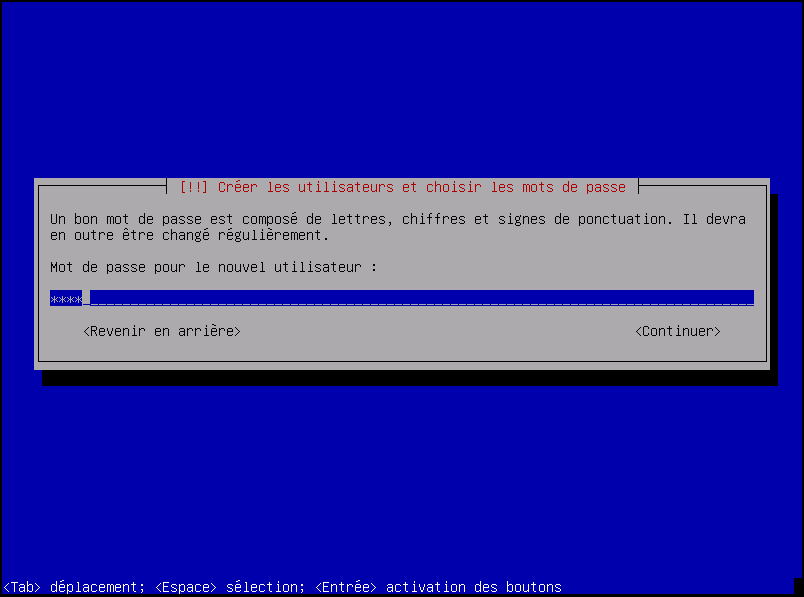
\includegraphics[scale=0.35]{img/install/Deb_inst_8.png}
 \caption{Création d'un utilisateur avec son mot de passe}
\end{figure}
\begin{figure}
 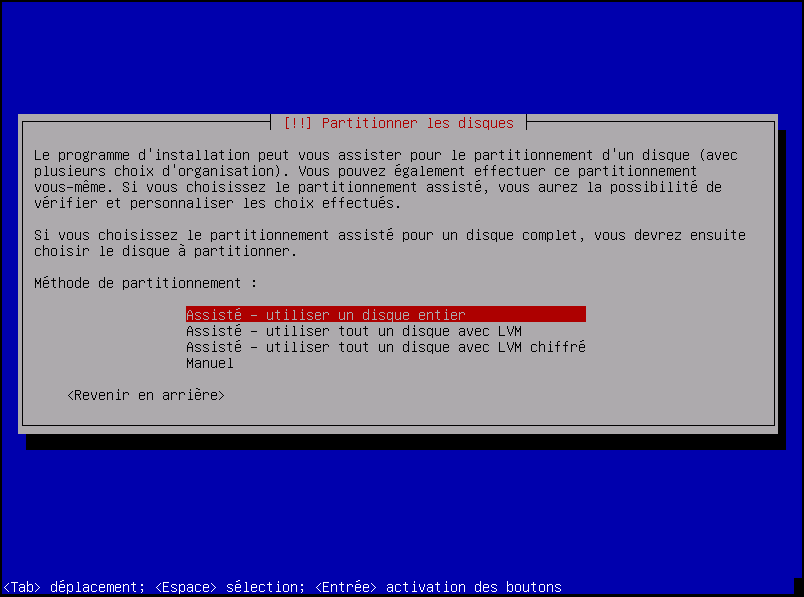
\includegraphics[scale=0.35]{img/install/Deb_inst_9.png}
 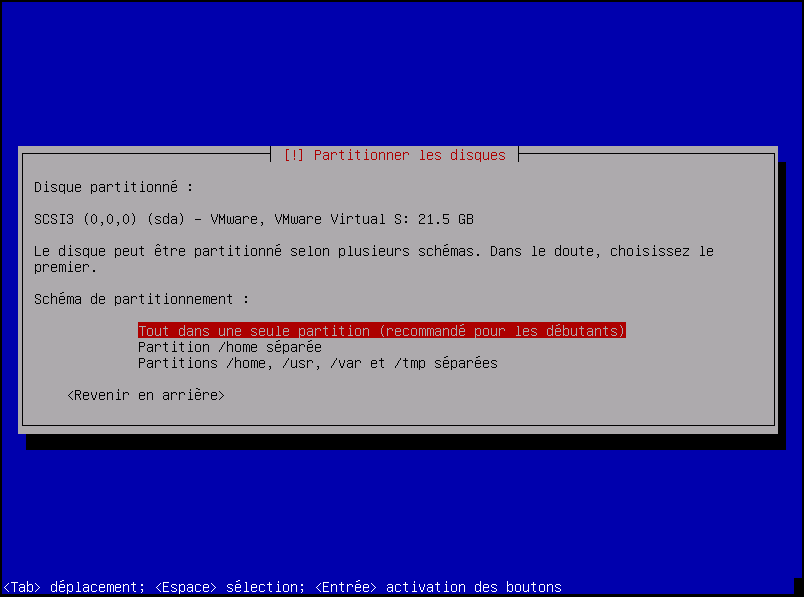
\includegraphics[scale=0.35]{img/install/Deb_inst_11.png}
 \caption{Partitionnement du disque dur et choix d'emplacement d'installation}
\end{figure}
\begin{figure}
 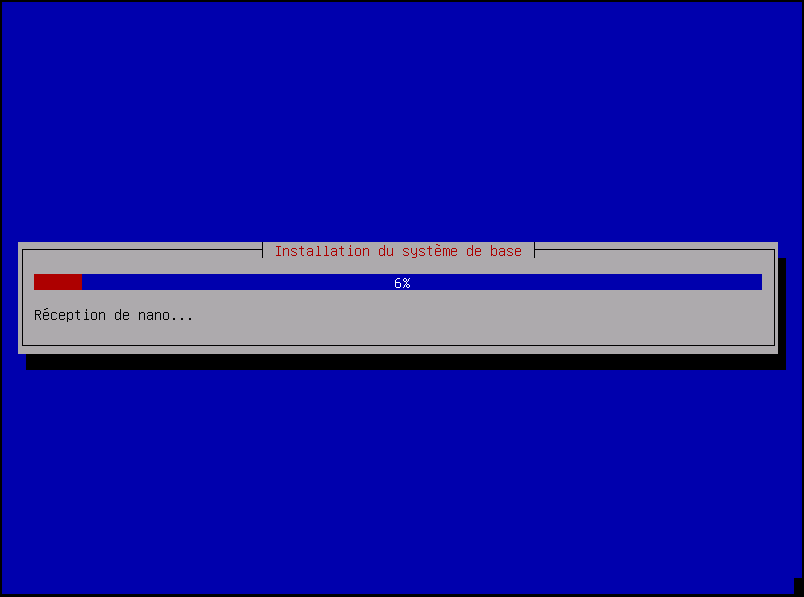
\includegraphics[scale=0.35]{img/install/Deb_inst_13.png}
 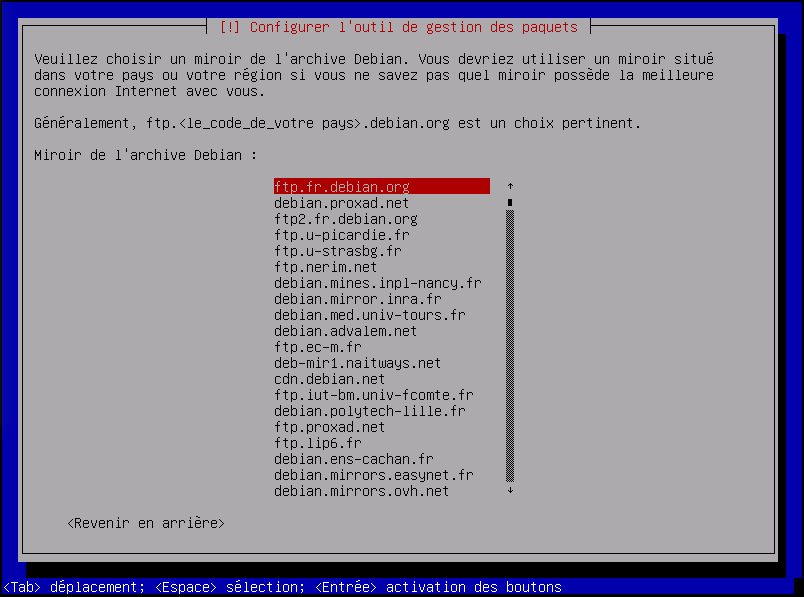
\includegraphics[scale=0.35]{img/install/Deb_inst_14.png}
 \caption{Installation du système et configuration des miroirs de packets}
\end{figure}
\begin{figure}
 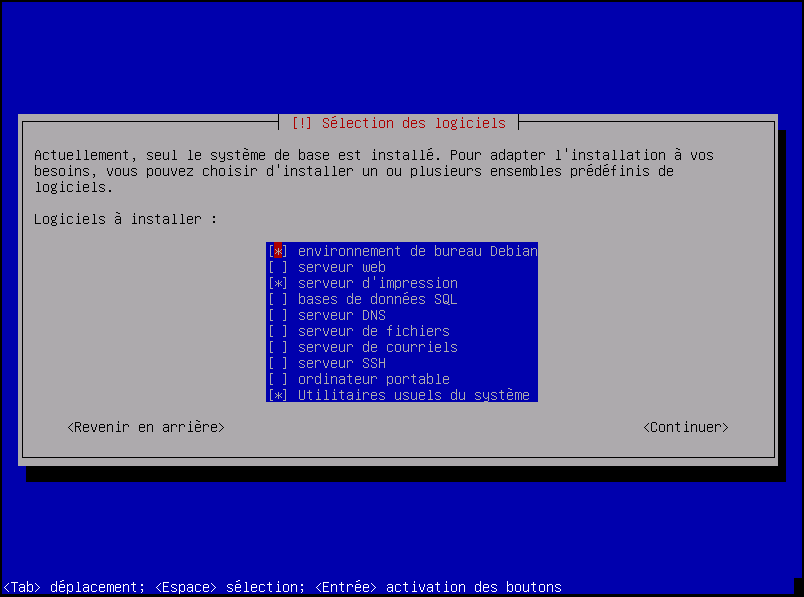
\includegraphics[scale=0.35]{img/install/Deb_inst_15.png}
 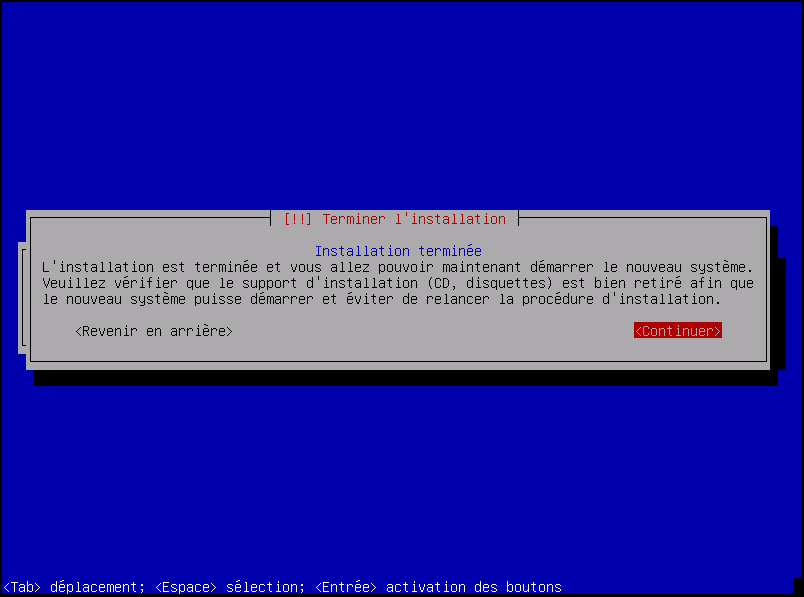
\includegraphics[scale=0.35]{img/install/Deb_inst_16.png}
 \caption{Choix des logiciels importants et finalisation de l'installation}
\end{figure}
\begin{figure}[h]
\centering
 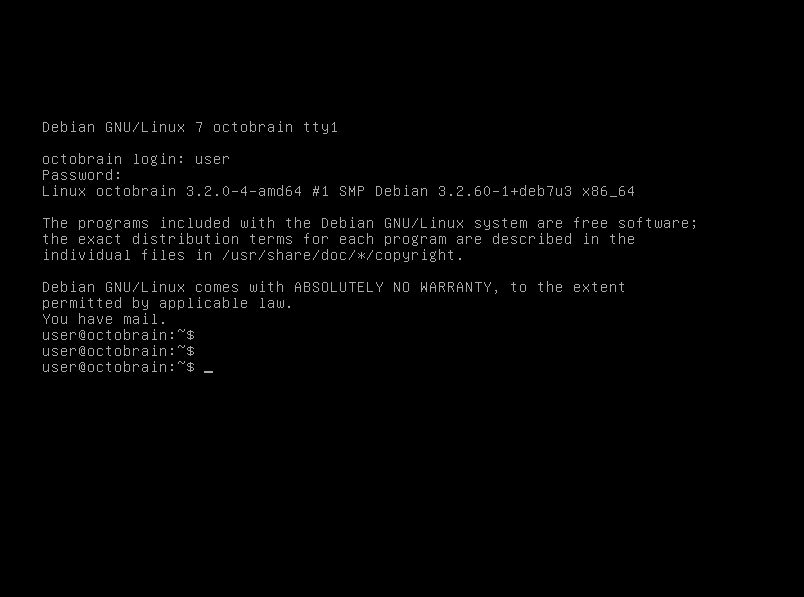
\includegraphics[scale=0.5]{img/install/Deb_inst_17.png}
 \caption{Ecran du système fonctionnel}
\end{figure}

\paragraph{}
Nous avons maintenant une machine virtuelle fonctionnant avec Debian 7 en installation minimale. C'est-à-dire que seul les packages essentiels sont installés. 
Afin de faire fonctionner correctement Octopus Supervisor, il faut ajouter les paquets suivants : gcc, make, libssl-dev, libsqlite3-dev.


\subsection{Installation d'un Xubuntu}
\paragraph{}
Nous allons vous montrer ci-dessous les différentes étapes d'une installation graphique du système Xubuntu.

\begin{figure}[h]
 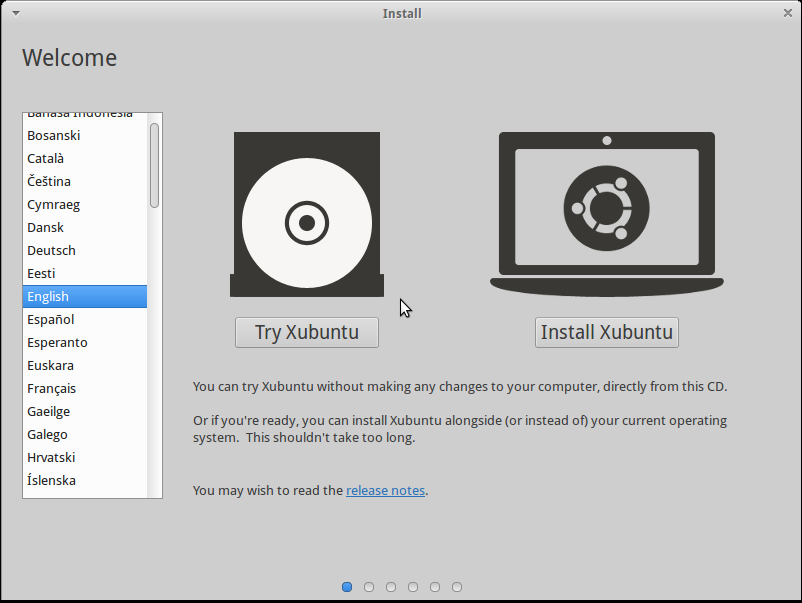
\includegraphics[scale=0.38]{img/install/Xub_inst_1.png}
 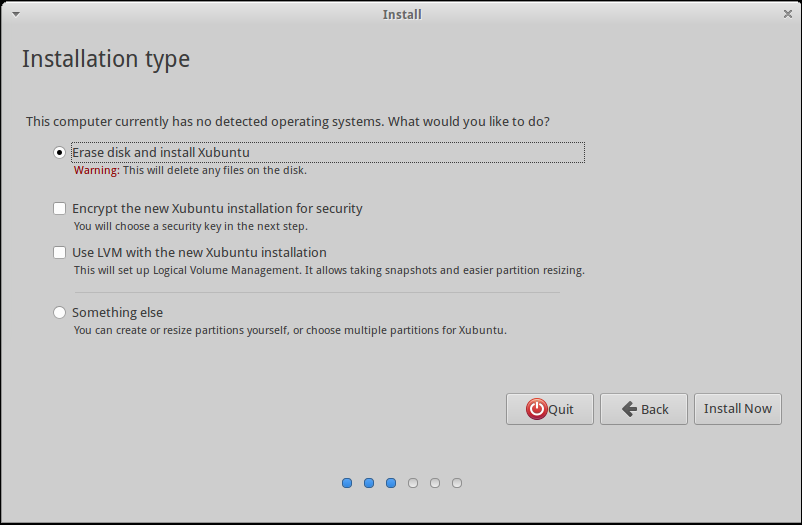
\includegraphics[scale=0.38]{img/install/Xub_inst_2.png}
 \caption{Choix de la langue et du type d'installation}
 \end{figure}
 \begin{figure}[h]
 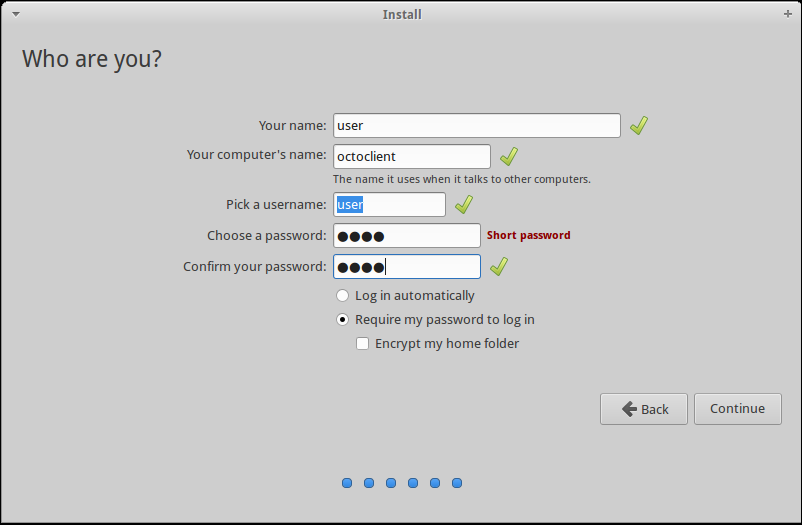
\includegraphics[scale=0.38]{img/install/Xub_inst_3.png}
 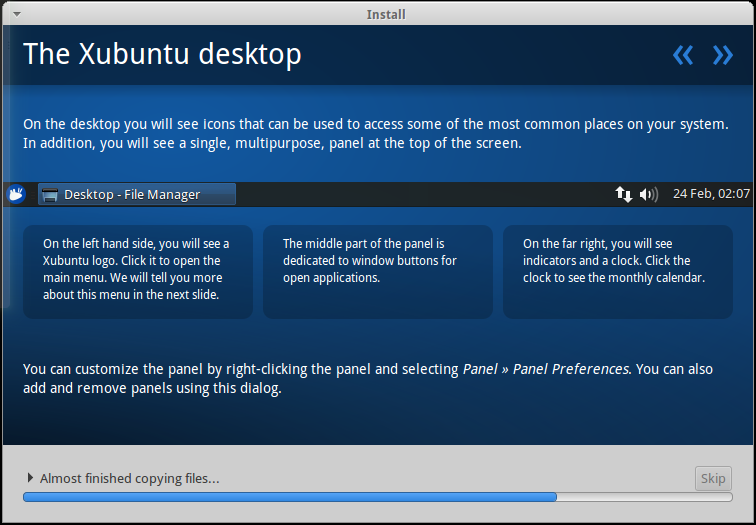
\includegraphics[scale=0.38]{img/install/Xub_inst_4.png}
 \caption{Définition d'un utilisateur et installation du système}
 \end{figure}
 \begin{figure}[h]
 \centering
 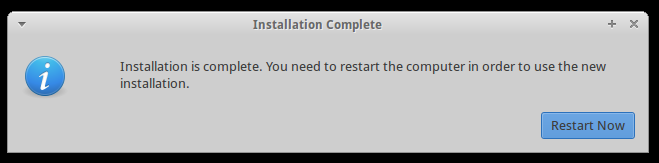
\includegraphics[scale=0.5]{img/install/Xub_inst_6.png}
 \caption{Fin de l'installation}
 \end{figure}
 \begin{figure}[h]
 \centering
 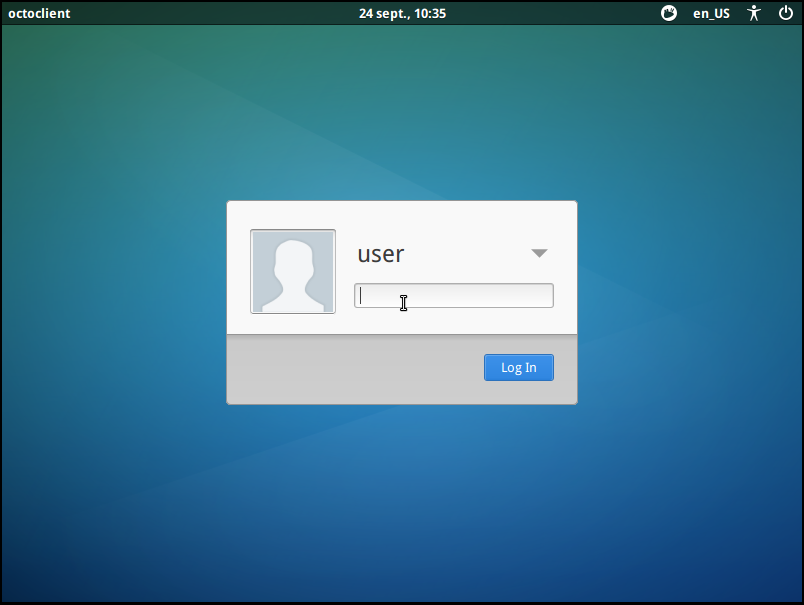
\includegraphics[scale=0.5]{img/install/Xub_inst_7.png}
 \caption{Ecran de connexion utilisateur}
 \end{figure}
 
 \paragraph{}
 Maintenant, nous avons un client opérationnel sous Xubuntu. Et nous pouvons ensuite installer le paquet client d'Octopus Supervisor.
 
\include{octopus-git}
\include{octopus-readme}

\listoffigures

\end{document}
